%%%%%%%%%%%%%%%%%%%%%%%%%%%%%%%%%%%%%%%%%%%%%%%%%%%%%%%%%%%%%%%%%%%%%%%%%%%%%%%%%%%%%%%%%%%%%%%%%%%%%%%
%%													%%
%% 	BAKALÁŘSKÁ PRÁCE - Zásuvný modul QGIS pro slučování vektorových map 				%%
%% 				 Tereza Fiedlerová							%%
%%													%%
%% pro formátování využita šablona: http://geo3.fsv.cvut.cz/kurzy/mod/resource/view.php?id=775 	%%
%%													%%
%%%%%%%%%%%%%%%%%%%%%%%%%%%%%%%%%%%%%%%%%%%%%%%%%%%%%%%%%%%%%%%%%%%%%%%%%%%%%%%%%%%%%%%%%%%%%%%%%%%%%%% 

\documentclass[%
  12pt,         			% Velikost základního písma je 12 bodů
  a4paper,      			% Formát papíru je A4
  twoside,       			% Oboustranný tisk
  pdftex				    % překlad bude proveden programem 'pdftex' do PDF
]{report}       			% Dokument třídy 'zpráva'
%

\usepackage[czech, english]{babel}	% použití češtiny, angličtiny
\usepackage[utf8x]{inputenc}		% Kódování zdrojových souborů je UTF8

\usepackage[square,sort,comma,numbers]{natbib}

\usepackage{caption}
\usepackage{subcaption}
\captionsetup{font=small}
\usepackage{enumitem} 
\setlist{leftmargin=*} % bez odsazení

\makeatletter
\setlength{\@fptop}{0pt}
\setlength{\@fpbot}{0pt plus 1fil}
\makeatletter

\usepackage[dvips]{graphicx}   
\usepackage{color}
\usepackage{transparent}
\usepackage{wrapfig}
\usepackage{float} 

\usepackage{cmap}           
\usepackage[T1]{fontenc}    

\usepackage{textcomp}
\usepackage[compact]{titlesec}
\usepackage{amsmath}
\addtolength{\jot}{1em} 

\usepackage{chngcntr}
\counterwithout{footnote}{chapter}

\usepackage{acronym}

\usepackage[
    unicode,                
    breaklinks=true,        
    hypertexnames=false,
    colorlinks=true, % true for print version
    citecolor=black,
    filecolor=black,
    linkcolor=black,
    urlcolor=black
]{hyperref}         

\usepackage{url}
\usepackage{fancyhdr}

\usepackage[
  cvutstyle,          
  bachelor           
]{thesiscvut}


\newif\ifweb
\ifx\ifHtml\undefined % Mimo HTML.
    \webfalse
\else % V HTML.
    \webtrue
\fi 

\renewcommand{\figurename}{Obrázek}
\def\figurename{Obrázek}

%%%%%%%%%%%%%%%%%%%%%%%%%%%%%%%%%%%%%%%%%%%%%%%%%%%%%%%%%%%%%%%%%
%%%%%%%%%%% Definice informací o dokumentu  %%%%%%%%%%%%%%%%%%%%%
%%%%%%%%%%%%%%%%%%%%%%%%%%%%%%%%%%%%%%%%%%%%%%%%%%%%%%%%%%%%%%%%%

%% Název práce
\nazev{název práce}{ EN title}

%% Jméno a příjmení autora
\autor{Martin}{Jákl}

%% Jméno a příjmení vedoucího práce včetně titulů
\garant{Ing. Martin Landa, PhD.}

%% Označení oboru studia
\oborstudia{Geoinformatika}{}

%% Označení ústavu
\ustav{Katedra  ??  }{}

%% Rok obhajoby
\rok{2016}

%Mesic obhajoby
\mesic{červen}

%% Místo obhajoby
\misto{Praha}

%% Abstrakt
\abstrakt 
{czech/ abstrakt}%
{english/ abstract}

%% Klíčová slova
\klicovaslova
{OSM, import, IPR, python, GDAL, GIS, .. klíčová slova}%
{OSM, import, IPR, python, GDAL,...... key words}

%%%%%%%%%%%%%%%%%%%%%%%%%%%%%%%%%%%%%%%%%%%%%%%%%%%%%%%%%%%%%%%%%%%%%%%%

%%%%%%%%%%%%%%%%%%%%%%%%%%%%%%%%%%%%%%%%%%%%%%%%%%%%%%%%%%%%%%%%%%%%%%%%
%% Nastavení polí ve Vlastnostech dokumentu PDF
%%%%%%%%%%%%%%%%%%%%%%%%%%%%%%%%%%%%%%%%%%%%%%%%%%%%%%%%%%%%%%%%%%%%%%%%
\nastavenipdf
%%%%%%%%%%%%%%%%%%%%%%%%%%%%%%%%%%%%%%%%%%%%%%%%%%%%%%%%%%%%%%%%%%%%%%%

%%% Začátek dokumentu
\begin{document}

\catcode`\-=12  % pro vypnuti aktivniho znaku '-' pouzivaneho napr. v \cline 

% aktivace záhlaví
\zahlavi

% předefinování vzhledu záhlaví
\renewcommand{\chaptermark}[1]{%
	\markboth{\MakeUppercase
	{%
	\thechapter.%
	\ #1}}{}}

% Vysázení přebalu práce
%\vytvorobalku

% Vysázení titulní stránky práce
\vytvortitulku

% Vysázení listu zadani
\stranka{}%
	{\sffamily\Huge\centering\ ZDE VLOŽIT LIST ZADÁNÍ}%
	{\sffamily\centering Z~důvodu správného číslování stránek}

% Vysázení stránky s abstraktem
\vytvorabstrakt

% Vysázení prohlaseni o samostatnosti
\vytvorprohlaseni

% Vysázení poděkování
\stranka{%nahore
       }{%uprostred
       }{%dole
       \sffamily
	\begin{flushleft}
		\large
		\MakeUppercase{Poděkování}
	\end{flushleft}
	\vspace{1em}
		%\noindent
	\par\hspace{2ex}
	{Chtěl bych poděkovat vedoucímu mé bakalářské práce, Ing. Martinu Landovi, PhD. ,
	za odborné rady a~pomoc při zpracování této práce. Dále bych chtěl 
	poděkovat své rodině za projevenou podporu a~trpělivost.}
}

% Vysázení obsahu
\obsah

% Vysázení seznamu obrázků
\seznamobrazku

% Vysázení seznamu tabulek
%\seznamtabulek

% jednotlivé kapitoly
\chapter{Úvod}
\label{1-uvod}

K projektu OpenStreetMap (OSM) jsem se dostal již před několika lety.
Zaujala mě možnost sám tvořit a upravovat \uv{mapu}.
Přidávat nové infomace ze svého okolí vlastním sběrem dat
a poté využívat takto vytvořenou mapu.

Postupem času jsem zjistil, co je, a co již není vhodné vkládat do mapy.
Když mi bylo na Fakultě stavební ČVUT v Praze nabídnuto vypracovat
bakalářskou práci na téma, které se dotýká problematiky datových importů OSM,
neváhal jsem. Nedávno totiž Institut plánování a rozvoje hlavního města Prahy
(IPR) uveřejnil všechna svá geografická data.
Tím vznikla možnost začlenit další vhodná data do projektu OSM.

Obsahem této práce je čtenáře nejprve seznámit s projektem
OpenStreetMap. Přiblížit mu vznik a vývoj projektu, užití a jeho licenci.
%%% ML: tato veta nedava smysl, co jste chtel presne rici
Jendá se o cíl, kam se budou importovat zpracovaná data z IPR.
Dále přiblížit problematiku datových importů do OSM a vysvětlit
pojem otevřená data (Open Data).

V praktické části navrhnout aplikaci v programovacím jazyce Python,
která by data poskytovaná IPR umožnila dávkově stáhnout a následně
importovat do pracovní geodatabáze PostGIS a popsat ovládání
vytvořené aplikace.

Následně provést rešerši zveřejněných dat IPR a porovnat je s daty,
která již jsou v OSM. Navrhnout, jaká data by byla vhodná importovat.
V průběhu práce konzultovat tento záměr s~komunitou OSM.
Nakonec vybraná data připravit k~importu z~geodatabáze PostGIS
do OSM.

\chapter{OpenStreetMap}% je videt
\label{2-OpenStreetMap}


\section{Vznik}
\label{vznik}
OpenStreetMap (OSM) je projekt, jež vznikl s cílem vytvoření a sběru 
volně dostupných geografických dat a následně jejich možné vizualizace
do topografických map. Projekt založil Steve Coast v červenci roku 
2004 v Anglii. Jako inspiraci mu byl projekt Wikipedia. 

Zprvu projekt využívalo jen pár nadšenců, ale postupem času získal 
projekt popularitu. S nárůstem počtu uživatelů narůstal i objem dat. 
Bylo tedy nutné zvyšovat kapacitu serverů. 

V dubnu roku 2006 byla založena nadace OpenStreetMap fundantion pro financováni 
samotného OSM (zaměstnanců, běhu serverů atd.). 
%\cite{wikiOSM}


\section{Struktura dat}
\label{struktura dat}

OSM data jsou ukládána ve formátu XML (verze 1.0). Jeho výhoda je jasná 
struktura, snadná orientace v kódu pro člověka. Nevýhodou je ovšem větší objem 
dat, který lze ale snížit kompresí. 

Každý prvek má vlastní XML soubor. 

příklad XML souboru pro linii:
...
.
.
%\lstset{language=XML}
%\begin{lstlisting}
%<osm version="0.6" generator="CGImap 0.4.0 (32632 thorn-01.openstreetmap.org)"copyright="OpenStreetMap and contributors" attribution="http://www.openstreetmap.org/copyright" license="http://opendatacommons.org/licenses/odbl/1-0/">
%    <way id="87249754" visible="true" version="2" changeset="34489106" timestamp="2015-10-07T11:52:41Z" user="Petr Dlouhý" uid="17615">
%        <nd ref="1014526199"/>
%        <nd ref="1014525941"/>
%        <nd ref="1014526337"/>
%        <nd ref="1014526022"/>
%        <nd ref="1014526277"/>
%        <nd ref="1014525984"/>
%        <tag k="highway" v="path"/>
%        <tag k="source" v="bing:ortofoto"/>
%    </way>
%</osm>
%\end{lstlisting}
.
.

Třídy prvků v OSM jsou rozděleny na uzel (node), cesta (way), polygon
(polygon) a všechny tyto prvky lze dále spojit do relace (relation).

Uzel je definován jedinečným identifikátorem (node id=). Jeho 
souřadnice jsou ve WGS~­84. Je také ukládána verze (version) a kdy 
byl do databáze přidán a v jaké změně to bylo provedeno (changeset=). 
Dále k bodu je možná připojit různé atributy s klíčem a hodnotou (tag~
k=~~v=~~). 

Linie je spojení dvou a více uzlů a má taky svůj identifikátor (way~
id=). Hlavičku má shodnou s bodem. Ale obsahuje také seznam id uzlů, 
jež ji tvoří. Liniím lze jí taktéž přiřadit atributy.  

Polygon je tvořen uzavřenou linií. Lze mu přiřadit jak liniové  atributy tak 
také atributy pro plochy. 

Speciálním příkladem jsou relace (relation=*), do které lze zahrnout 
jeden a více prvků. Lze do nich spojit prvky stejné nebo odlišné třídy 
nebo i jiné relace. Pro příklad dálnice je tvořena mnoha liniemi a ty 
jsou zahrnuty do společné relace Dálnice D1. Nebo turistická trasa 
(od~KČT) je relace sdružující linie (cesty, pěšiny) tak i uzly 
(rozcestníky, vyhlídky, apod. ).

U atributů popsaných na osmwiki je vždy uvedeno, k jaké třídě je 
vhodné a nevhodné je použít (dle komunity uživatelů OSM). Pokud se stane, že je použit 
na~jinou než povolenou třídu, nemusí to hlásit chybu, ale může být následně 
problém v některých vykreslovačích. 

\section{Licence}
\label{licence}

Původní data OSM byla na distribuována pod licencí 
Creative~Commons~Allribution­Share~Alike 2.0 (CC~BY~­SA~2.0). 
(Lincence CC~BY~SA~2.0 zní:  „ ... “  )

Tato licence umožňovala užití (distribuci ale i editaci) díla pod podmínkou, 
že bude uveden zdroj OpenStreetMap.org ve viditelné části 
vytvořených mapových dlaždic [?2] 

  \begin{figure}[hbt]
    \centering
      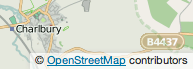
\includegraphics{./pictures/attribution_example.png}
      \caption{attribution example}
      \label{fig:attribution_example}
  \end{figure} 

Roku 2012 byla licence publikovaných dat změněna na Open Data Commons 
Open Database Licence (OdbL). Tato změna licence přinesla problém 
s~daty, které byly poskytnuty projektu v předchozí licencí 
(CC­~BY~SA~2.0). Bylo nutné se dotázat každého z dřívějších 
přispěvatelů dat, ať už právnických osob tak i fyzických osob, jestli 
s touto změnou souhlasí a je možné s jejich daty i s novou licencí 
nakládat. U přispěvatelů, kteří nedovolili užívání jejich díla 
pod novou licencí, nebo u těch, co se nevyjádřili, bylo nutné 
z~databáze vymazat. Tato situace nastala pouze ve zlomku případů. 
Nejvíce tato změna licencí ohrozila data v zemích jako je Polsko a Nový Zéland.
 [?5] 

\section{Opendata}
\label{opendata}
Základní myšlenka otevřených dat vznikla v USA z iniciativy vlády Barracka Obamy. 
Tedy, pokud vzniknou geografická data z veřejných peněz, měla by tedy být přístupná 
veřejně. Mělo to kladný efekt na tamní ekonomiku.
Díky tomuto byly zprvu k dispozici satelitní snímky povrchu 
Země a digitální model terénu s rozlišením 30x30 m od NASA (pro 
pozdější vykreslení vrstevnic). 

Tento trend se začal rozšiřovat zprvu do zemí západních Evropy,
jmenovitě Anglie, Francie, ale i jiné země mimo Evropu..  

V ČR se tomuto věnuje fond otevrenadata.cz, který založil Otakar 
Motejl. Teto fond spolupracuje s nadací Sociery Fund Praha. V rámci 
těchto uskupení je vyvíjen tlak na zveřejňování smluv a dat 
státních institucí, jelikož jejich získání a údržba bylo placeno 
z~veřejných zdrojů.

\section{Zdroje dat}
\label{opendata}

Jak bylo zmíněno, byla snaha aby mapová data tvořili jedinci, vlastním 
sběrem dat. Sběr dat ve smyslu měřením vlastní GNSS (GPS, Glonass) 
přijímačem a znalost místních poměrů (uzavřené silnice, stezky atd.). 
Toto mapové dílo z těchto dat mohli volně užívat k vlastním užití. 
Komunita přispěvatelů se zprvu pomalu, ale později rychle rozrostla a 
dnes čítá 3,7 milionů registrovaných uživatelů s alespoň jednou 
vytvořenou změnou v OSM a 2,7 milionů účtů aktivních přispěvatelů.

Tyto mapové podklady byly velice vhodné i pro další projekt, dnes již 
velice rozšířený a známý jako Geocashing (GC). Projekt GC začal mapové 
podklady od OSM užívat a zároveň jeho uživatelé začali sami tvořit a 
přispívat do OSM. 

Přispěvatelé dat do OSM musí respektovat, že OSM je pod licencí OdbL. 
Tudíž i jejich zdroj dat musí splňovat tuto licenci. Proto by měli 
všechny svoje změny, které v OSM vytvoří, řádně ozdrojovat atributem 
s~klíčem 
source=*
V případě vlastním sběrem dat se vyplňuje hodnotou 
source=survey
případně uvést zdroj, odkud čerpali. Pokud tuto povinnost poruší a 
použijí zdroj, jež není kompatibilní z politikou OSM, tak samotné OSM 
jejich změnu, aby předešel sporům, sám vymaže. Bohužel musí vymazat 
celou sadu změn, byť by v něm byl jeden prvek, jež toto poruší. 

Druhým významným zdrojem dat jsou soukromé subjekty (společnosti). 
V~tomto případě jde většinou o podkladové zdroje dat. Pro obkreslování 
silničních síti z~leteckých nebo satelitních rastrů. V~jejich případě 
řešeno písemným svolením, nebo smlouvou. Jako významným zdrojem byla 
společnost Bing, jež nabídla k~dispozici letecké snímky většiny 
obydlené pevniny. 

Třetím zdrojem a zároveň postupně dominujícím co do obsahu dat, jsou 
databáze ze státního sektoru. Tyto databáze jsou nejvhodnějším zdrojem 
dat. Data v nich jsou důkladně spravována už proto, že je využívá stát. 

\section{Vykreslovače}
\label{vykreslovače}
Na hlavní stránce OSM je pět „základních“ přednastavených vrstev vykreslených 
z~dat z OSM. Využívá aplikaci OpenLayers založenou na konceptu AJAX.

\begin{itemize}

  \item Standardní vrstva - vykresluje všechny prvky přiměřeně.
  \item Cyklomapa - vykresluje cyklostezky, výškopis. 
  \item Dopravní mapa - vykresluje silniční a železniční sítě.
  \item MapQuest Open vznikla jako podkladová mapa právě pro potřeby 
Geocaching.
  \item Humanitární mapa, která vykresluje služby (restaurace, banky, muzea, 
  školy, kostely...)  a potlačuje ostatní prvky 

\end{itemize}

Existují další stránky jež se zabývají vlastní kompozicí a vykreslením
různých dat. Například mapu turistických a cyklistických tras vykresluje
 mtbmap.cz a to pro celou Evropu. 
 
Zajímavými projekty jsou, které k 2D mapě přidává „třetí“ rozměr a 
vytváří tzv. 2.5D mapu. Většinou jde o 3D zobrazení budov, mostů (dle 
atributů) popřípadě i stromů. 


\chapter{Importy}% je videt
\label{2-importy}

Hromadné datové importy do OSM jsou cenným zdrojem dat. V rámci České 
republiky proběhlo již několik dávkových importů. Většina z nich byla 
začlenění dat ze státních databází. Hlavní výhoda je jejich celistvost 
v rámci státu nebo oblasti, nevýhodou může být ne vždy aktuálnost 
informací. Některá data mohou být sbírána a zveřejněna i s delším 
časovým odstupem.   

Samotný proces importu vykonají stoje respektive výpočetní technika a 
není to tedy moc náročné na čas a lidské zdroje jako samotný sběr. 
Avšak větší časovou náročnost zabere příprava, a to jak samotných dat 
nebo napsání programu (skriptu) tak i probrání problematiky s~komunitou OSM. 

Větší čas zabere vybrat, jaká data jsou vhodná a přínosná. Prozkoumat 
zdali již nejsou v databázi částečně zanesena od jednotlivých 
uživatelů vlastním sběrem dat. Není příliš vhodné odstraňovat z mapy 
něco, co tam některý uživatel s~velkým úsilím zanesl. Také se může 
stát, že uživatel se znalostní místních poměrů bude vědět více, jak se 
věci mají v jeho okolí, něž-­li uživatel dělajíc import od stolu 
(například malé vodní toky, jejichž koryto se hýbe). Proto se volí 
řešení s~vytvořením duplicit. Je totiž snažší odstranit duplicitně 
vloženou správnou informaci, než-li po vymazání původní a nahrání nové 
řešit, že ta původní jedna byla správně. Toto lze řešit, kdyby tato 
jedna změna byla v jednom changelist­-u. Tuto změnu by bylo možné 
vrátit, což v řešení hromadných importů, kdy je mnoho změn, není 
možné.

Je tedy nutné zvážit velikost takto vytvořených duplicit. A rozhodnout 
jak postupovat při jejich pozdějším řešením. Zdali autor původních dat 
nečerpal ze stejného zdroje nebo zdali nejsou staršího data a bude 
tedy snadné vyřešit, která data ponechat. 

Je taky potřeba řešit otázku „tagování“. Problém pravděpodobně nebude 
přiřadit hlavní atribut dané „věci“ (například 
„řeka“~~waterway=river“) ale atributy, jež nejsou v mapě 
vykreslovány, ale odliší od sebe prvky nebo je zařadí do společné 
oblasti (atribut is\-in, city.. atd). Toto je vhodné nejprve vyřešitpo 
poradě s komunitou OSM na diskuzi task­osm.cz

\section{Licenční otázka}
\label{2-Importy}

Po vyřešení otázky, která data začlenit do databáze OSM a s jakým 
klíčem, je také nutné vyřešit licenční otázky. Není určeno, v jakém 
pořadí by se mělo toto řešit. Je spíše vhodné řešit nejprve licenční podmínky. 
Zdali autor nebo vlastník je nakloněn myšlence opendata.  

Pokud by například vlastník dat, která chce zveřejnit nebo již 
zveřejnil, nebyla pod licencí kompatibilní s OSM. Tedy nebyla by 
pod~licencí ODbL. Tento problém leze řešit tak, že buď by se počkalo
na~změnu licence nebo by se musela udělit speciální výjimka pro OSM.
Bohužel by tato výjimka  problém neřešila, jelikož byla data z OSM dále
distribuována pod licencí ODbL. Lepším řešení je zveřejňovat otevřená
data pod vícero licencemi. Popřípadě pod licencí, která je „kompatibilní“ 
s~ostatními nebo s~předchozími. Například CC­~BY~SA~4.0 je zpětně kompatibilní 
s~licencemi ...   ale zpětně to nemusí platit.  



%\include{9-zaver}

% Vysázení seznamu zkratek
%\begin{seznamzkratek}{ABCDE}

    \novazkratka{OSM}
		{OSM}
		{OpenStreetMap (\textit{Open Street Map})}

    \novazkratka{IPR}
	    {IPR}
        {Institut plánování a rozvoje hlavního města Prahy}

    \novazkratka{RUIAN}
	    {RUIAN}
        {Registr územní identifikace, adres a nemovitostí}

    \novazkratka{PID}
	    {PID}
        {Pražská integrovaná doprava}

    \novazkratka{KČT}
	    {KČT}
        {Klub českých turistů}

    \novazkratka{CC-BY-SA}
		{CC-BY-SA}
		{Uveďte původ-Zachovejte licenci (\textit{Creative Commons Attribution-ShareAlike})}

    \novazkratka{ODbL}
		{ODbL}
		{(\textit{Open Database License})}

    \novazkratka{GIS}
	      {GIS}
 	      {Geografický informační systém  (\textit{Geographic Information System})}

    \novazkratka{GNSS}
		{GNSS}
		{Globální družicový polohový systém (\textit{Global Navigation Satellite System})}

    \novazkratka{GPS}
		{GPS}
		{Globální polohovací systém (\textit{Global Positioning System})}

    \novazkratka{GLONASS}
		{GLONASS}
		{Glonass (\textit{Globalnaja navigacionnaja sputnikovaja sistěma})}

    \novazkratka{WGS 84}
		{WGS 84}
		{Světový geodetický systém 1984 (\textit{World Geodetic System 1984})}

    \novazkratka{S-JTSK}
		{S-JTSK}
		{Systém jednotné trigonometrické sítě katastrální}

    \novazkratka{GC}
		{GC}
		{Geocaching (\textit{Geocaching})}

    \novazkratka{SQL}
		{SQL}
		{SQL (\textit{Structured Query Language})}

    \novazkratka{XML}
		{XML}
		{Rozšiřitelný značkovací jazyk (\textit{Extensible Markup Language})}

    \novazkratka{GDAL}
		{GDAL}
		{Geoprostorová datová knihovna (\textit{Geospatial Data Abstraction Library})}

    \novazkratka{QGIS}
        {QGIS}
        {Quantum GIS}

    \novazkratka{JOSM}
        {JOSM}
        {Java OpenStreetMap Editor}


\end{seznamzkratek}


% Literatura
\nocite{*}
\def\refname{Literatura}
\bibliographystyle{mystyle}
%\bibliography{literatura}


% Začátek příloh
%\prilohy

% Vysázení seznamu příloh
%\seznampriloh

% Vložení souboru s přílohami
%\chapter{Typy vykreslení OSM dat}
\label{vykresleni_dat}

\begin{figure}[H]
    \centering
    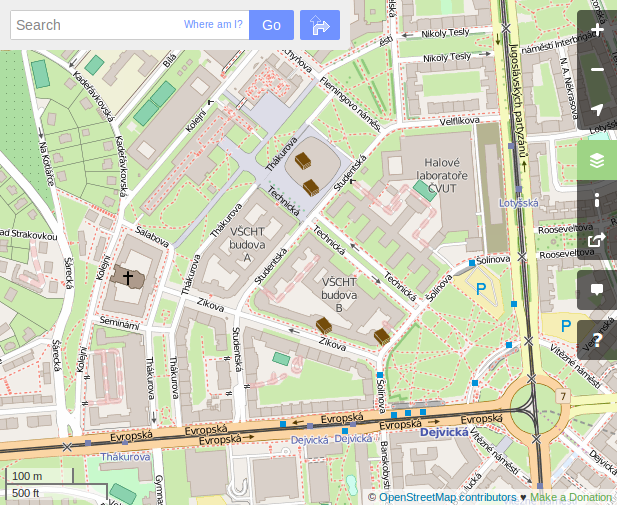
\includegraphics[width=11.5cm]{pictures/osm_standard.png} 
    \caption{Standardní mapa (Standard)}
    \label{fig:standard}
\end{figure}

\begin{figure}[H]
    \centering
    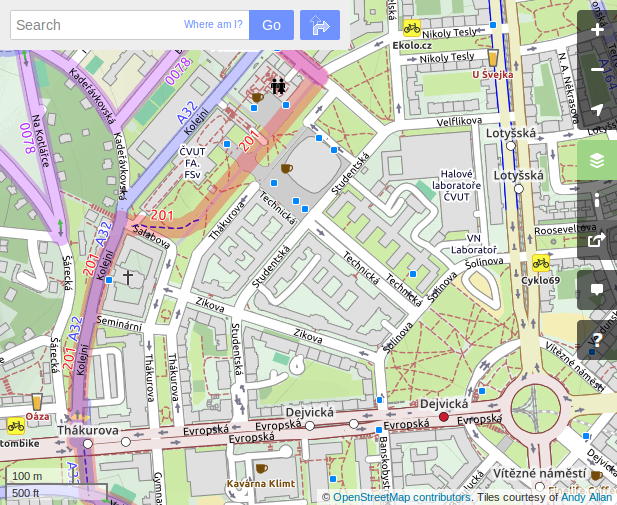
\includegraphics[width=11.5cm]{pictures/osm_cyclemap.png} 
    \caption{Cyklistická mapa (Cycle Map)}
    \label{fig:cycle}
\end{figure}

% new list

\begin{figure}[H]
    \centering
    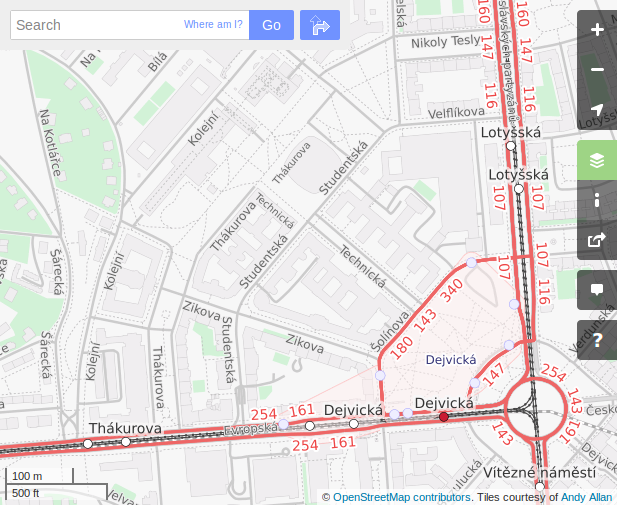
\includegraphics[width=11.5cm]{pictures/osm_transport.png} 
    \caption{Transport Map}
    \label{fig:transport}
\end{figure}

\begin{figure}[H]
    \centering
    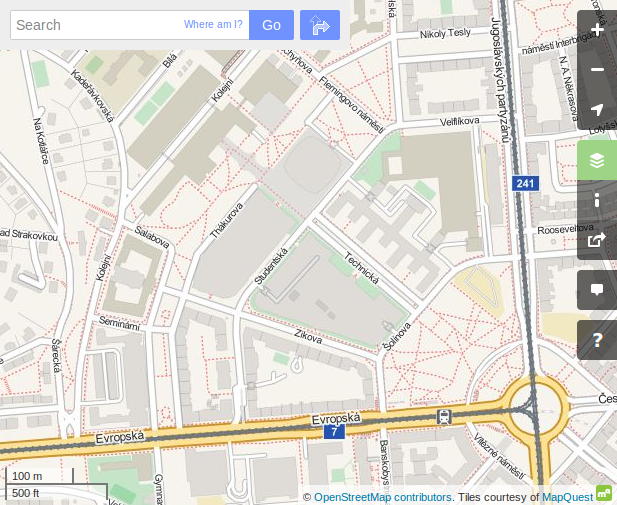
\includegraphics[width=11.5cm]{pictures/osm_mapquest.png} 
    \caption{MapQuest Open}
    \label{fig:mapquest}
\end{figure}

% new list

\begin{figure}[H]
    \centering
    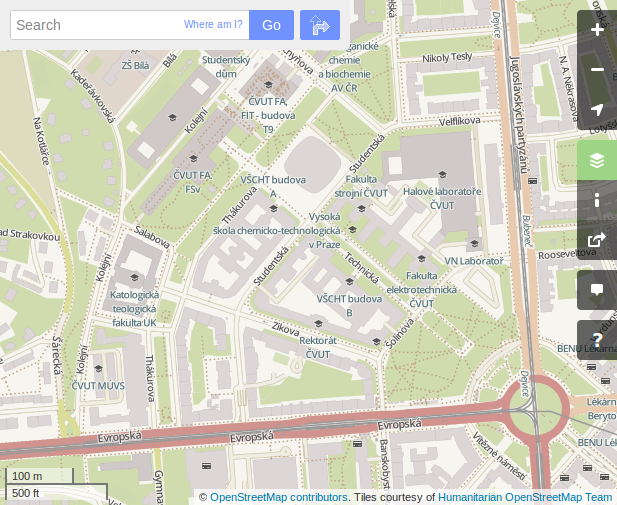
\includegraphics[width=11.5cm]{pictures/osm_humanitarian.png} 
    \caption{Humanitární mapa (Humanitarian)}
    \label{fig:humanitarian}
\end{figure}

\begin{figure}[H]
    \centering
    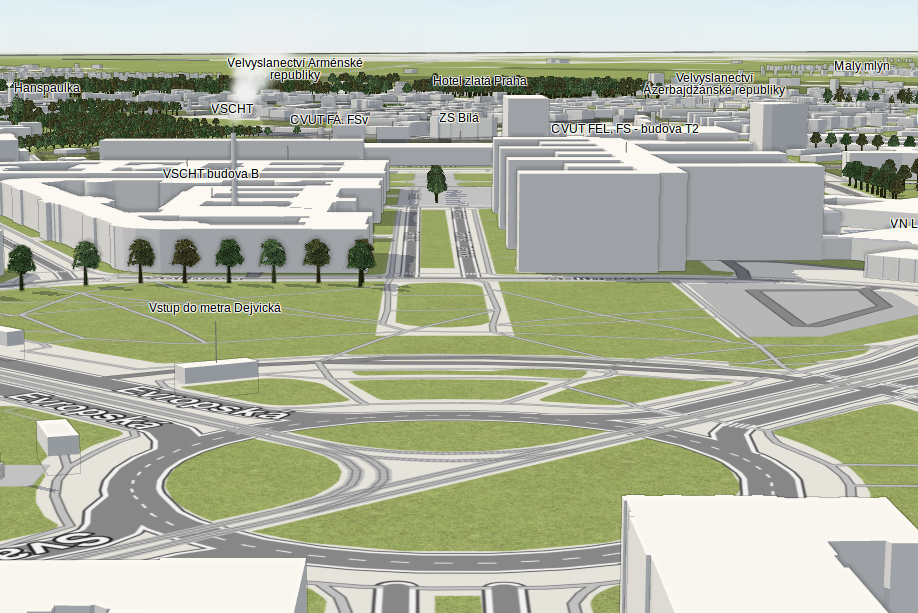
\includegraphics[width=11.5cm]{pictures/F4.png} 
    \caption{projekt F4 (zdroj \url{http://demo.f4map.com/}}
    \label{fig:F4}
\end{figure}

% new list

\chapter{Diagramy}
\label{digramy}

\begin{figure}[H]
  \centering
  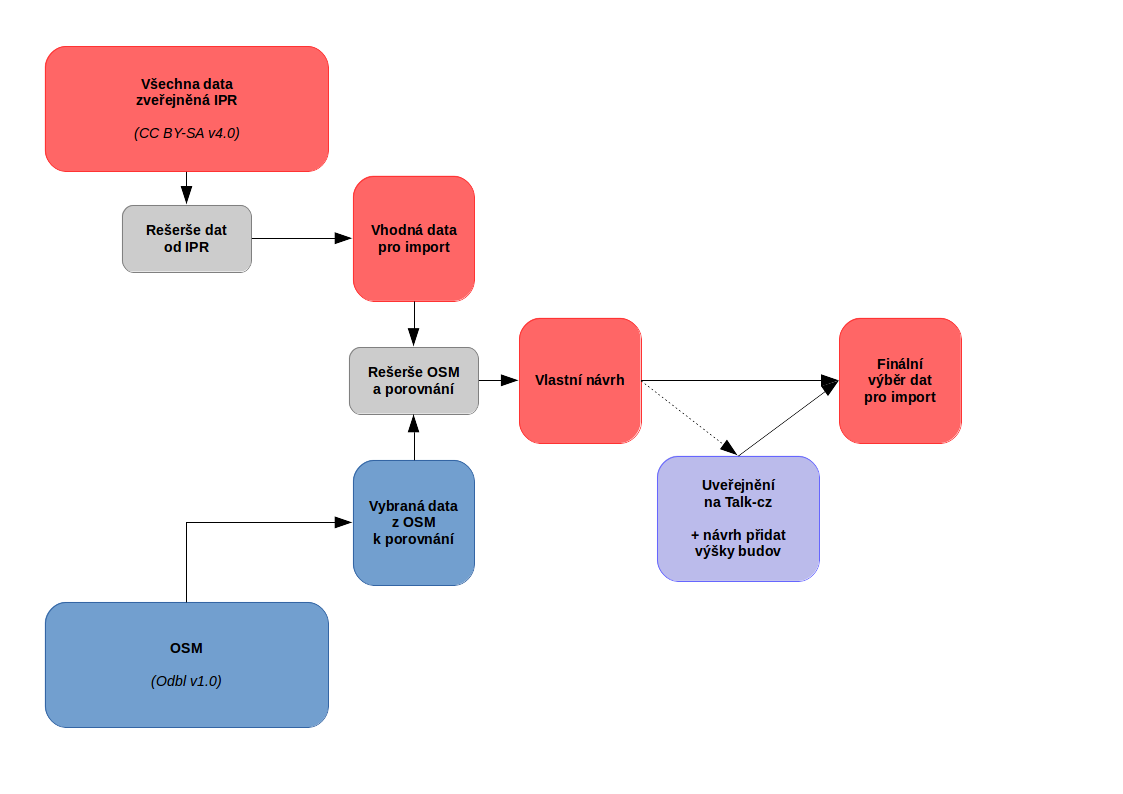
\includegraphics[scale=0.60,angle=90]{pictures/WorkFlow.png}
  \caption{Diagram postupu práce.}
  \label{fig:diagram_workflow}
\end{figure}

\begin{figure}[H]
  \centering
  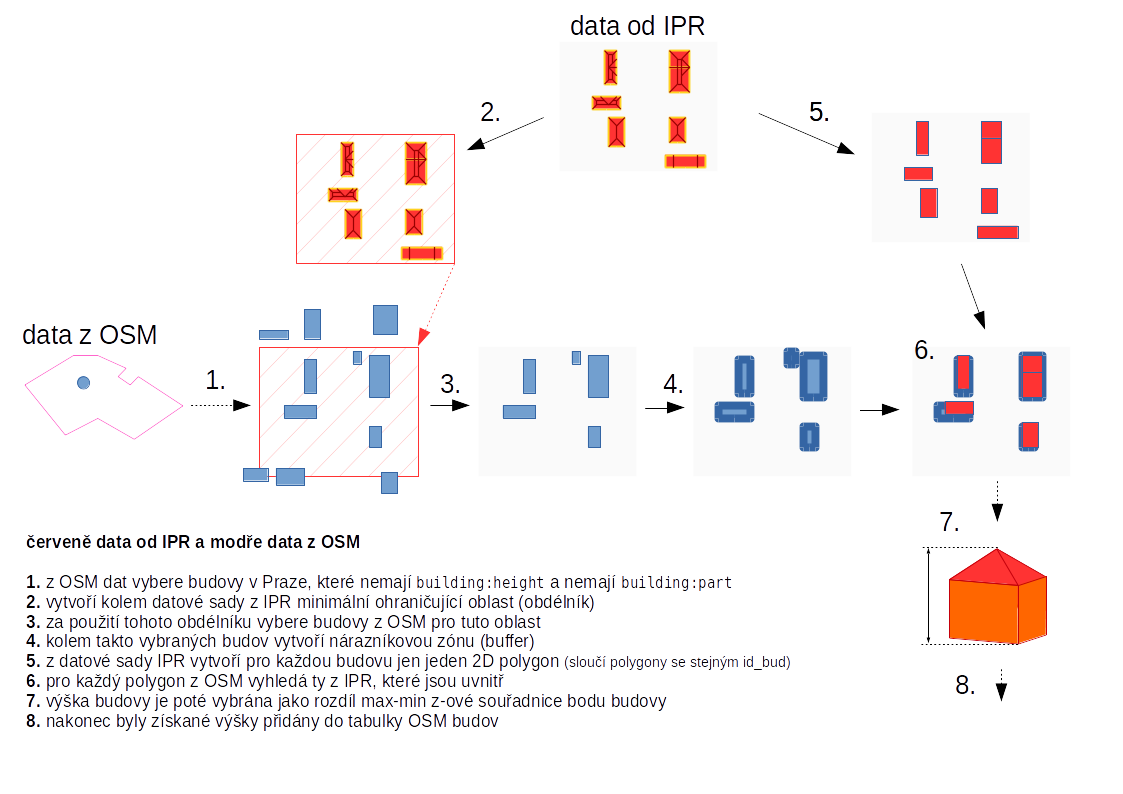
\includegraphics[scale=0.60,angle=90]{pictures/diagram_building_height.png}
  \caption{Diagram postupu práce pro získání výšky budov.}
  \label{fig:diagram_building}
\end{figure}

% new list

\chapter{Obsah CD}
\label{priloha-obsahCD}
\setlength{\unitlength}{.5mm}
\begin{picture}(250, 220)

  \put(  0, 212){\textbf{.}}

  \put(  1, 200){\line(0, 1){5}}
  \put(  1, 200){\line(1, 0){10} {\textbf{ src}}}  

      \put( 16, 190){\line(0, 1){8}}
      \put( 16, 190){\line(1, 0){10} {\textbf{ iprdownloader}}}
      \put(150, 190){ zdrojové soubory programu}

          \put( 29, 180){\line(0, 1){8}}
          \put( 29, 180){\line(1, 0){10} { IprBase.py}}
          \put( 29, 170){\line(0, 1){10}}
          \put( 29, 170){\line(1, 0){10} { IprPg.py}}
          \put( 29, 160){\line(0, 1){10}}
          \put( 29, 160){\line(1, 0){10} {\textbf{ Iprdownloader.py}}}

      \put( 16, 150){\line(0, 1){40}}
      \put( 16, 150){\line(1, 0){10} {\textbf{ pg}}}
      \put(150, 150){ zdrojové kódy shell skriptu}      

          \put( 29, 140){\line(0, 1){8}}
          \put( 29, 140){\line(1, 0){10} { pgis\_osm\_bp.style}}
          \put(150, 140){ vlastní schema dat z OSM}
          \put( 29, 130){\line(0, 1){10}}
          \put( 29, 130){\line(1, 0){10} { upgrade\_pgis\_osm\_bp.sql}}
          
      \put( 16, 120){\line(0, 1){30}}
      \put( 16, 120){\line(1, 0){10} {\textbf{ sql}}}
      \put(150, 120){ zdrojové kódy sql dump}
            
          \put( 29, 110){\line(0, 1){8}}
          \put( 29, 110){\line(1, 0){10} { buildins.sql}}
          \put( 29, 100){\line(0, 1){10}}
          \put( 29, 100){\line(1, 0){10} { park\_and\_ride.sql}}
          \put( 29,  90){\line(0, 1){10}}
          \put( 29,  90){\line(1, 0){10} { parkomat.sql}}
          \put( 29,  80){\line(0, 1){10}}
          \put( 29,  80){\line(1, 0){10} { recycling\_centre.sql}}
          \put( 29,  70){\line(0, 1){10}}
          \put( 29,  70){\line(1, 0){10} { toilets.sql}}          
          
  \put(  1,  60){\line(0, 1){140}}
  \put(  1,  60){\line(1, 0){10} {\textbf{ text}}}

      \put( 16,  50){\line(0, 1){8}}
      \put( 16,  50){\line(1, 0){10} {\textbf{ latex}}}
      \put(150,  50){ zdrojové soubory textu této práce}
      \put( 16,  40){\line(0, 1){10}}
      \put( 16,  40){\line(1, 0){10} { martin-jakl-bp-2016.xls}}
      \put(150,  40){ anotace práce}
      \put( 16,  30){\line(0, 1){10}}
      \put( 16,  30){\line(1, 0){10} { martin-jakl-bp-2016.pdf}}
      \put(150,  30){ tento text}
      \put( 16,  20){\line(0, 1){10}}
      \put( 16,  20){\line(1, 0){10} { zadani-oficialni.jpeg}}
      \put(150,  20){ naskenované oficiální zadání práce}
\end{picture}


% Konec dokumentu
\end{document}
